%\title{EMC LaTeX Portrait Poster Template}
%%%%%%%%%%%%%%%%%%%%%%%%%%%%%%%%%%%%%%%%%
% a1poster Portrait Poster
% LaTeX Template
% Version 2.0 (22/06/16)
%
% The a1poster class was created by:
% Joe Rowing (JoeRowing@exeterms.ac.uk)
% 
% This template has been produced by:
% Joe Rowing at Exeter Mathematics School
%
% License:
% CC BY-NC-SA 3.0 (http://creativecommons.org/licenses/by-nc-sa/3.0/)
%
%%%%%%%%%%%%%%%%%%%%%%%%%%%%%%%%%%%%%%%%%

%----------------------------------------------------------------------------------------
%   PACKAGES AND OTHER DOCUMENT CONFIGURATIONS
%----------------------------------------------------------------------------------------

\documentclass[a1,portrait]{a1poster}

\usepackage{multicol} % This is so we can have multiple columns of text side-by-side
\columnsep=50pt % This is the amount of white space between the columns in the poster
\columnseprule=0.01pt % This is the thickness of the black line between the columns in the poster

\usepackage[svgnames]{xcolor} % Specify colors by their 'svgnames', for a full list of all colors available see here: http://www.latextemplates.com/svgnames-colors

\usepackage{times} % Use the times font


\usepackage{graphicx} % Required for including images
\graphicspath{{figures/}} % Location of the graphics files
\usepackage{booktabs} % Top and bottom rules for table
\usepackage[font=small,labelfont=bf]{caption} % Required for specifying captions to tables and figures
\usepackage{amsfonts, amsmath, amsthm, amssymb} % For math fonts, symbols and environments
\usepackage{wrapfig} % Allows wrapping text around tables and figures
\setlength{\parskip}{\baselineskip}%
\setlength{\parindent}{10pt}%

\begin{document}

%----------------------------------------------------------------------------------------
%   POSTER HEADER 
% The header is divided into two boxes:
% The first is 75% wide and houses the title, subtitle, names, university/organization and contact information
% The second is 25% wide and houses the EMS Logo
% 
%----------------------------------------------------------------------------------------

\begin{minipage}[b]{0.6\linewidth}
\Huge \color{DarkOliveGreen} \textbf{Statistical Survey and Analysis of Fireballs and NEOs} \color{Black}\\ % Title
%\huge\textit{With a subtitle here}\\[1cm] % Subtitle
\large \textbf{Hernández, Giovanna}\\[0.5cm] % Author(s)
\large Escuela de Ciencias Físicas y Matemáticas, Universidad de San Carlos de Guatemala\\[0.2cm] % University/organization
\texttt{gioreneeha@gmail.com}\\
\end{minipage}
%
\begin{minipage}[b]{0.4\linewidth}

\includegraphics[width=15cm]{ecfmLogoColorO.png}\\
\end{minipage}

\vspace{.5cm} % A bit of extra whitespace between the header and poster content

%----------------------------------------------------------------------------------------

\begin{multicols}{2} % This is how many columns your poster will be broken into, by convention a portrait poster is generally split into 2 or 3 columns

%----------------------------------------------------------------------------------------
%   ABSTRACT

%An abstract is a brief summary of a research article, thesis, review, conference proceeding or any in-depth analysis of a particular subject and is often used to help the reader quickly ascertain the paper's purpose
%----------------------------------------------------------------------------------------

\color{DarkOliveGreen} % Colour for the abstract

% \begin{abstract}

%     \large{Studying Near-Earth Objects (NEOs) and fireballs is incredibly important for
%     understanding the potential threats that these objects pose to our planet. This article 
%     presents the statistical survey and analysis of fundamental parameters of a sample of NEOs
%     and fireballs obtained from the database of The Center for Near-Earth Object Studies (CNEOS),
%     where it was examined the distributions and correlations of key parameters including impact
%     energy, impact probability, absolute magnitude and geographic location of these phenomena.
%     The results of this study contribute to a deeper understanding of these astronomical objects
%     and their potential impact on Earth.}

% \end{abstract}

\section*{Abstract}

Studying Near-Earth Objects (NEOs) and fireballs is incredibly important for
understanding the potential threats that these objects pose to our planet. This article 
presents the statistical survey and analysis of fundamental parameters of a sample of NEOs
and fireballs obtained from the database of The Center for Near-Earth Object Studies (CNEOS),
where it was examined the distributions and correlations of key parameters including impact
energy, impact probability, absolute magnitude and geographic location of these phenomena.
The results of this study contribute to a deeper understanding of these astronomical objects
and their potential impact on Earth.

%----------------------------------------------------------------------------------------
%   INTRODUCTION

%Avoid using technical definitions unless absolutely necessary. The introduction section is here to introduce your issue, so be sure to not bore your readers right away with excessive information. You can even include graphics if they will help the viewer understand the work that you have done.
%----------------------------------------------------------------------------------------

\color{Black} % color for the introduction

\section*{Introduction}

Near-Earth Objects (NEOs) are comets and asteroids that have been nudged by the gravitational
attraction of nearby planets into orbits that allow them to enter the Earth’s neighborhood. Composed
mostly of water ice with embedded dust particles, comets originally formed in the cold outer planetary
system while most of the rocky asteroids formed in the warmer inner solar system between the orbits of
Mars and Jupiter.  \cite{nasaBasics}

A meteoroid is generally defined as an asteroid or comet fragment that orbits the Sun. Meteors, or
"shooting stars", are the visible paths of meteoroids that have entered the Earth’s atmosphere at high
velocities. A fireball is an unusually bright meteor that reaches a visual magnitude of $-3$ or
brighter when seen at the observer’s zenith. \cite{nasaFireballs}

Near-Earth Asteroids (NEAs) are small bodies of the Solar System with perihelion distance $q$
$1.3\:AU$ (Astronomical Units) and aphelion distances $Q$ $0.983\:AU$, whose orbits approach or
intersect Earth orbit. \cite{rukmini2016statistical} Potentially Hazardous Asteroids (PHAs) are a
special subset of NEAs that, according to The Center for Near-Earth Object Studies (CNEOS), have an
absolute magnitude ($H$) of $22.0$ or less that can come close to the Earth and are large enough to
cause significant damage in the event of an impact. \cite{zhou2024martians}

Sentry is a highly automated collision monitoring system that continually scans the most current
asteroid catalog for possibilities of future impact with Earth over the next 100 years. Whenever a
potential impact is detected it will be analyzed and the results immediately published, except in
unusual cases. \cite{nasaSentryEarth}

%----------------------------------------------------------------------------------------
%   OBJECTIVES
%----------------------------------------------------------------------------------------

\color{Black} % DarkSlateGray color for the rest of the content

\section*{Data and Methods}

The data about fireballs, NEOs, NEAs and impact probabilities have been collected from the database of
The Center for Near-Earth Object Studies (CNEOS) and its monitoring system Sentry. The parameters
studied include absolute visual magnitude ($H$), impact probability, impact energy ($kt$) and
geographic location of fireball objects.

To determine if the impact energy ($kt$) of fireballs is consistent with some type of distribution it
was decided to use the logarithm of the data and then a histogram was made with the counts of the
impact energy ($log(kt)$) in intervals of $0.2$. With these data, some distribution fit were applied
to confirm wich one was more accurate.

At first, the covariance matrix was used to find the linear bond between NEOs absolute magnitude ($H$)
and impact probability, but due to the correlation not being linear, it was discarded. Then proceeded
to use Pearson and Spearman correlation coefficients to analyze better the data and determine if a
correlation existed and which type it was.

At last, using Gnuplot and Python with various libraries such as pandas, numpy, plotly, a graphic
representation of geographic locations with their respective impact energy as the size of the reported
events was made.

%----------------------------------------------------------------------------------------
%   RESULTS 

%It’s always a good idea to begin the Results section with an initial summary of your results. Don’t address your research question just yet; instead, just address the general aspects of the data you collected or the number of valid data obtained.

%In your next paragraph, you can discuss the relationship between the data and your research question. What exactly does your data mean? Be sure to include any graphics that can help show you data visually, as the readers can understand graphics more easily and quickly than blocks of text.

%Sometimes less is more. Be selective when deciding what images, charts, and graphs make it onto your poster! 

%Charts and graphs are usually more effective than tables, but whatever you choose to use, make sure everything is labeled clearly! A graph with missing labels or a table without a title will just leave the reader confused. Also, carefully consider what type of chart or graph will best show your results. K. Broman, professor of Biostatistics & Medical Informatics at the University of Wisconsin Madison has written a great article titled, “The Top Ten Worst Graphs.” (http://www.biostat.wisc.edu/~kbroman/topten_worstgraphs/)
%----------------------------------------------------------------------------------------

\section*{Results}

\begin{center}\vspace{1cm}
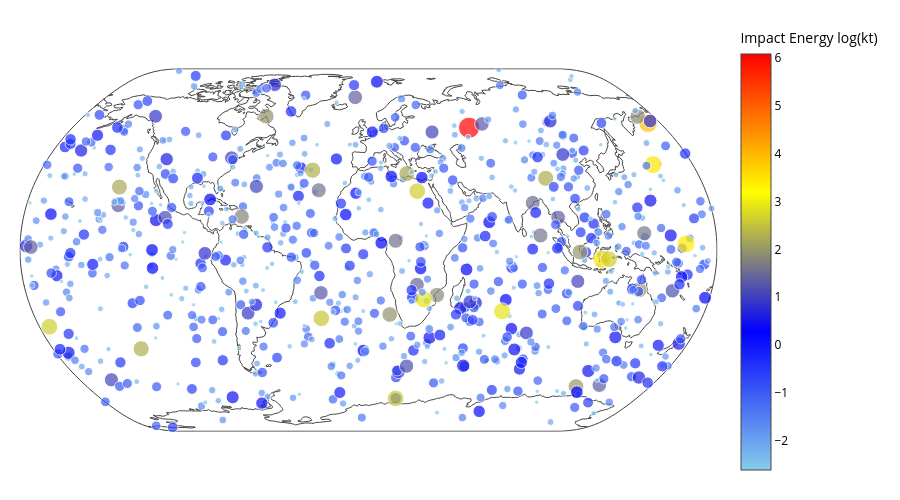
\includegraphics[width=0.8\linewidth]{fireballs}
\captionof{figure}{Fireballs reported by US government sensors from April 15, 1988, to May 15, 2024. The size and color of each circle were determined by the logarithm of the impact energy (kt), and the location was determined by the altitude and longitude. All this data was obtained from the database published by NASA’s CNEOS at JPL.}
\label{fig:fireballs}
\end{center}\vspace{1cm}

As it can be observed in figure \ref{fig:fireballs} and figure \ref{fig:gaussian}, the most frequent
impact energy is $-2.4$ to $-2.2$ $log(kt)$ which is equivalent to $0.09$ and $0.11$ $kt$. Little
data varies from $1$ to $3$ $log(kt)$, or its equivalent range $2.72$ to $20.01$ $kt$ And even more
impressive, only one data was far from the rest, it had an impact energy of $440$ $kt$. That piece of
information was unique among the rest, to the point where it's easy to tell from where the data is. It
was the Chelyabinsk meteor of February 15, 2013. It generated infrasound returns, after circling the
globe, at distances up to $\sim85000$ $km$, and was detected at $20$ infrasonic stations of the global
International Monitoring System (IMS). \cite{key} It was surely a unique occurrence.

In figure \ref{fig:gaussian} it can be seen that the fit of a Gaussian distribution was the best,
but it had a $\chi^2$ value of $6.37E+03$, which means that the fit had a large variation concerning
the original data. With this, it can be said that the fit wasn't precise. On the other hand, the Poisson
distribution was also used, but in that case, a fit was not even generated. Same case with Log-normal
distribution. That was the reason the Gaussian distribution was selected as the best-fitting
one, despite its high variation with the presented data.

\begin{center}\vspace{1cm}
    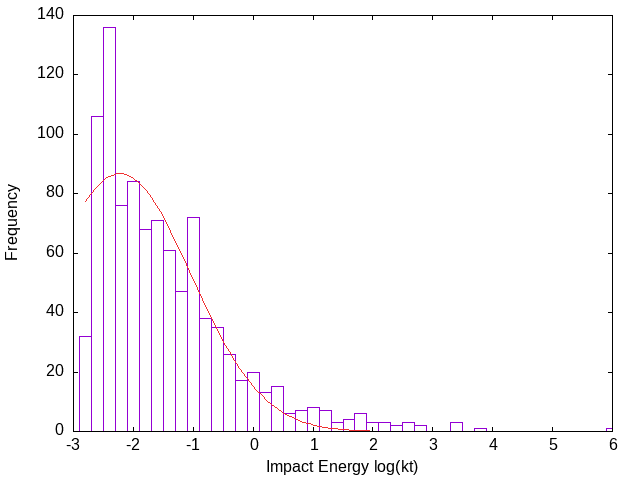
\includegraphics[width=0.5\linewidth]{fit}
    \captionof{figure}{Histogram of logarithmic fireballs impact energy ($kt$) reported by US government sensors from April 15, 1988, to May 15, 2024. The red line indicates the fit of a Gaussian distribution that was applied to the data. The larger impact energy was of $6\:log(kt)$.}
    \label{fig:gaussian}
\end{center}\vspace{1cm}

With figure \ref{fig:probability}, it can be observed the correlation between NEOs impact probability
and absolute magnitude ($H$). To analyze these data, Pearson and Spearman coefficients and the
covariance matrix were used. 

The diagonal of the covariance matrix had a value of $-4.28$ for non-cumulative probability and $1.72$
for cumulative probability. These results suggest that, in the first case, the two data had a negative
correlation, but, in the second case, they had a positive correlation, which is not coherent. For that
reason, the covariance matrix was the first method to be discarded.

Then Pearson coefficient was utilized. It gave a correlation of $-0.01$ for non-cumulative
probability and $0.34$ for cumulative probability. As in the previous instance, this suggests that
in the first case, the two data had a negative correlation and a positive one in the second case. This
occurs because both, the covariance matrix and the Pearson coefficient, expect that the data follows
a Gaussian or Gaussian-like distribution, which the presented data does not follow.

Finally, Spearman coefficient was used. It returned a correlation of $0.60$ for non-cumulative
probability and $0.81$ for cumulative probability. Unlike the previous ones, this test gave a
coherent number, which indicates that the data have a non-linear monotonic correlation.

\begin{center}\vspace{1cm}
    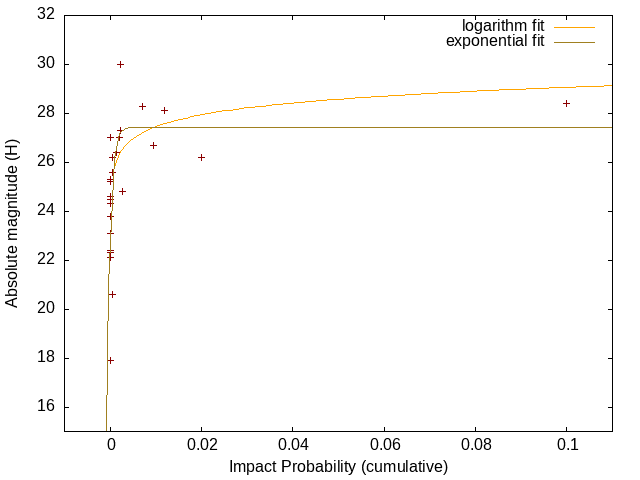
\includegraphics[width=0.5\linewidth]{correlation}
    \captionof{figure}{Plot between NEOs impact probability and absolute magnitude ($H$) obtained from the database published by NASA’s CNEOS at JPL. The olive line indicates an exponential fit and the yellow one indicates a logarithmic fit, both were applied to the data.}
    \label{fig:probability}
\end{center}\vspace{1cm}

The exponential fit, corresponding to the olive line in figure \ref{fig:probability}, had a $\chi^2$
value of $94.07$, and the logarithmic fit, corresponding to the yellow line in figure \ref{fig:probability},
had a $\chi^2$ value of $89.15$. In comparison, the logarithmic fit presented fewer variations with the
sample data, but it showed that none of them were able to fit correctly the correlation. Due to all of
the above, it can be said that there exists a non-linear monotonic correlation between NEO impact
probability and absolute magnitude ($H$), but it isn't enough to fit it into a function either in
logarithmic or exponential form.

Also, it can be noted that there exists an inverse correlation between the absolute magnitude ($H$) and
the diameter of astronomical objects. So it can be assumed that the impact probability has a small inverse
correlation with the diameter of the NEO. But the correlation isn't strong enough to extrapolate it
correctly.

%----------------------------------------------------------------------------------------
%   CONCLUSIONS
%In your conclusion section you want to briefly review your research questions and the results you obtain. You also should add why your results are interesting or significant. TIPS: Relate your results to other published research in the field. This will give your research more impact on your readers as well as show your professionalism in the study. You can also suggest continuing research that would build upon your current study.
%----------------------------------------------------------------------------------------

\color{DarkOliveGreen} %  colour for the conclusions to make them stand out

\section*{Conclusions}

\begin{itemize}
    \item The most likely impact energy of a fireball is between the range of $0.09$ and $0.11$ $kt$,
	being the ones with impact energy between $2.72$ and $20.01$ $kt$ a rare occurrence and
	a fireball with impact energy larger than $50$ $kt$ a unique event.
	\item Even though the figure \ref{fig:gaussian} resembles some kind of distribution, the ones that
	were fitted to the histogram didn't return precise fittings or a fit at all.
	\item From figure \ref{fig:probability} it can be observed that it's unlikely for a PHA to impact
	Earth. That's because according to CNEOS, the NEA should have an absolute magnitude ($H$) of $22.0$
	or less, and the graph shows that these kinds of objects are the ones with the least impact probability.
	\item It was shown that, according to various correlation coefficients, there exists a small non-linear
	monotonic relationship between the absolute magnitude ($H$) and the impact probability of NEO. But
	it isn't enough to extrapolate it to an inverse relationship between diameter and impact probability.
	\item Due to the particular correlation between the absolute magnitude ($H$) and the impact probability
	found in this study, the data can't be fitted into a function, either in logarithmic or exponential form.
	\item It can be concluded that the study of NEOs, NEAs, fireballs and more objects of this kind, it's
	extensive and of great interest to comprehend in a better way the behavior of these objects and their
	implications for the integrity of the Earth.
\end{itemize}

\color{Black} % Set the color back to DarkSlateGray for the rest of the content

%----------------------------------------------------------------------------------------
%   REFERENCES
%If you have an extremely extensive list of references, you may want to break it into 2 columns. 

% It is common to shrink the font of the References section if it becomes overbearing and long

%----------------------------------------------------------------------------------------
\begin{small}%Makes the text of the references section smaller
\begin{multicols}{2}%Makes the section two col
%\nocite{*} % Print all references regardless of whether they were cited in the poster or not
\bibliographystyle{plain} % Plain referencing style
\bibliography{bibliography} % Use the example bibliography file sample.bib
\end{multicols}
\end{small}
%----------------------------------------------------------------------------------------
%	 CONTACT DETAILS
%A lot of posters include this section so the readers are able to contact the author later or read more about the research. You can include your email or website address, links to relevant resources, or even a QR code (What is a QR Code?) that viewers can scan to go directly to your website or a PDF version of your poster. If you choose to include this section, keep it very brief
%----------------------------------------------------------------------------------------
\section*{Contact Details}
Giovanna Hernández - gioreneeha@gmail.com
\end{multicols}
\end{document}
